\documentclass[10pt,a4paper]{article}

\usepackage{fontspec}
\usepackage[spanish,es-noshorthands,es-tabla]{babel}
\usepackage[margin=1.8cm]{geometry}
\usepackage{graphicx}
\usepackage{booktabs}
\usepackage{float}
\usepackage{caption}
\usepackage{tikz}
\usetikzlibrary{arrows.meta,positioning}
\usepackage{titlesec}
\usepackage{enumitem}
\usepackage[hidelinks]{hyperref}

\graphicspath{{../../sims/lt3092/figures/}}
\captionsetup{font=small,labelfont=bf,skip=3pt}
\titlespacing*{\section}{0pt}{8pt}{4pt}
\titlespacing*{\subsection}{0pt}{6pt}{2pt}
\setlength{\parskip}{2pt}
\setlength{\textfloatsep}{8pt}
\setlength{\intextsep}{6pt}

\begin{document}

\begin{center}
{\Large\textbf{Simulación de la fuente de corriente IEPE del sonómetro}}\\[3pt]
Evaluación del LT3092 de Analog Devices \quad·\quad Proyecto Sonómetro IEPE \quad·\quad 27 de octubre de 2026
\end{center}

\section{Componente seleccionado}

Se eligió el \textbf{LT3092} de Analog Devices, una fuente de corriente ajustable de dos terminales: el fabricante la usa para alimentar sensores IEPE en su diseño de referencia CN0540, la corriente se fija con solo dos resistencias, admite hasta 40~V y viene en un encapsulado fácil de soldar (SOT-223). Las alternativas de Texas Instruments revisadas (TIDA-010249 y TIDA-01471) también son válidas, pero necesitan más componentes.

\section{Metodología}

Se simuló en LTspice con el modelo oficial del LT3092, automatizando las corridas con Python. El micrófono ROGA RG-50 se representó como su polarización de 12,5~V más la señal, en serie con su resistencia de salida de 50~$\Omega$. Como casos exigentes se usaron el nivel máximo del micrófono (130~dB, unos 3,5~V de señal) y su ruido propio (32~dB, unos 41~$\mu$V).

\begin{figure}[H]
\centering
\begin{minipage}[c]{0.56\textwidth}
\centering
\begin{tikzpicture}[
  bloque/.style={draw, rounded corners, minimum width=2.2cm, minimum height=0.9cm, align=center, font=\scriptsize},
  flecha/.style={-{Stealth[length=2mm]}, thick}]
  \node[bloque] (vin) {Alimentación\\24 V};
  \node[bloque, right=0.9cm of vin] (lt) {LT3092};
  \node[bloque, right=0.9cm of lt] (mic) {Micrófono\\RG-50};
  \node[bloque, below=0.7cm of mic] (ac) {Acoplamiento AC};
  \node[bloque, left=0.9cm of ac] (adc) {Conversión\\y análisis};
  \draw[flecha] (vin) -- (lt);
  \draw[flecha] (lt) -- node[above, font=\tiny]{2,8 mA} (mic);
  \draw[flecha] (mic) -- node[right, font=\tiny]{12,5 V + señal} (ac);
  \draw[flecha] (ac) -- node[above, font=\tiny]{señal} (adc);
\end{tikzpicture}
\captionof{figure}{Cadena simulada.}
\label{fig:esquema}
\end{minipage}\hfill
\begin{minipage}[c]{0.42\textwidth}
\centering
\captionof{table}{Corrientes evaluadas ($R_{SET} = 20$~k$\Omega$).}
\label{tab:corrientes}
\small
\begin{tabular}{lcc}
\toprule
Objetivo & $R_{OUT}$ & Simulada \\
\midrule
2,4 mA & 84,5 $\Omega$ & 2,377 mA \\
2,8 mA & 71,5 $\Omega$ & 2,808 mA \\
4,0 mA & 49,9 $\Omega$ & 4,019 mA \\
\bottomrule
\end{tabular}
\end{minipage}
\end{figure}

\section{Resultados}

\textbf{Tensión de alimentación (Fig.~\ref{fig:compliance}).} Con la señal máxima, la corriente se mantiene a partir de unos \textbf{17,6~V}. Con \textbf{24~V} queda un margen de 6,4~V, dentro del rango de 18 a 30~V que pide el micrófono.

\textbf{Señal fuerte (Fig.~\ref{fig:senal}).} Con 24~V la corriente varía solo un 0,08~\% ante un tono de 130~dB. Con 17~V la corriente cae casi a cero en los picos, lo que en el micrófono real sería una señal recortada.

\begin{figure}[H]
\centering
\begin{minipage}[t]{0.49\textwidth}
\centering
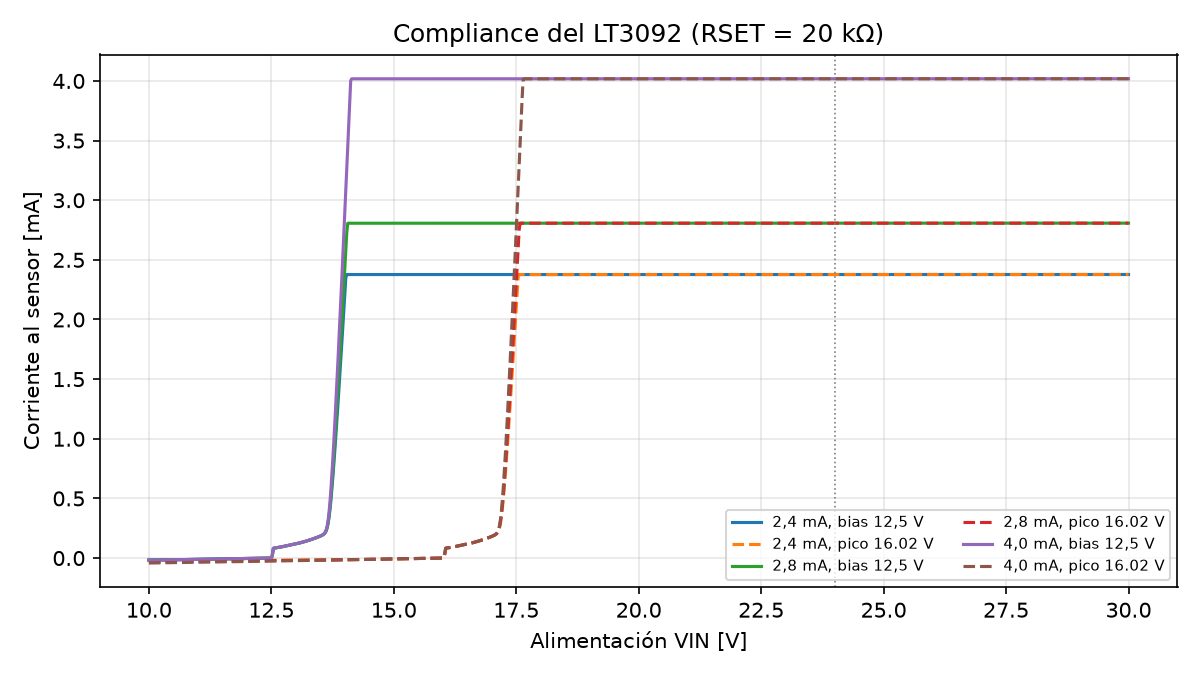
\includegraphics[width=\linewidth]{01_compliance.png}
\captionof{figure}{Corriente frente a la alimentación; en discontinuo, con la señal máxima.}
\label{fig:compliance}
\end{minipage}\hfill
\begin{minipage}[t]{0.49\textwidth}
\centering
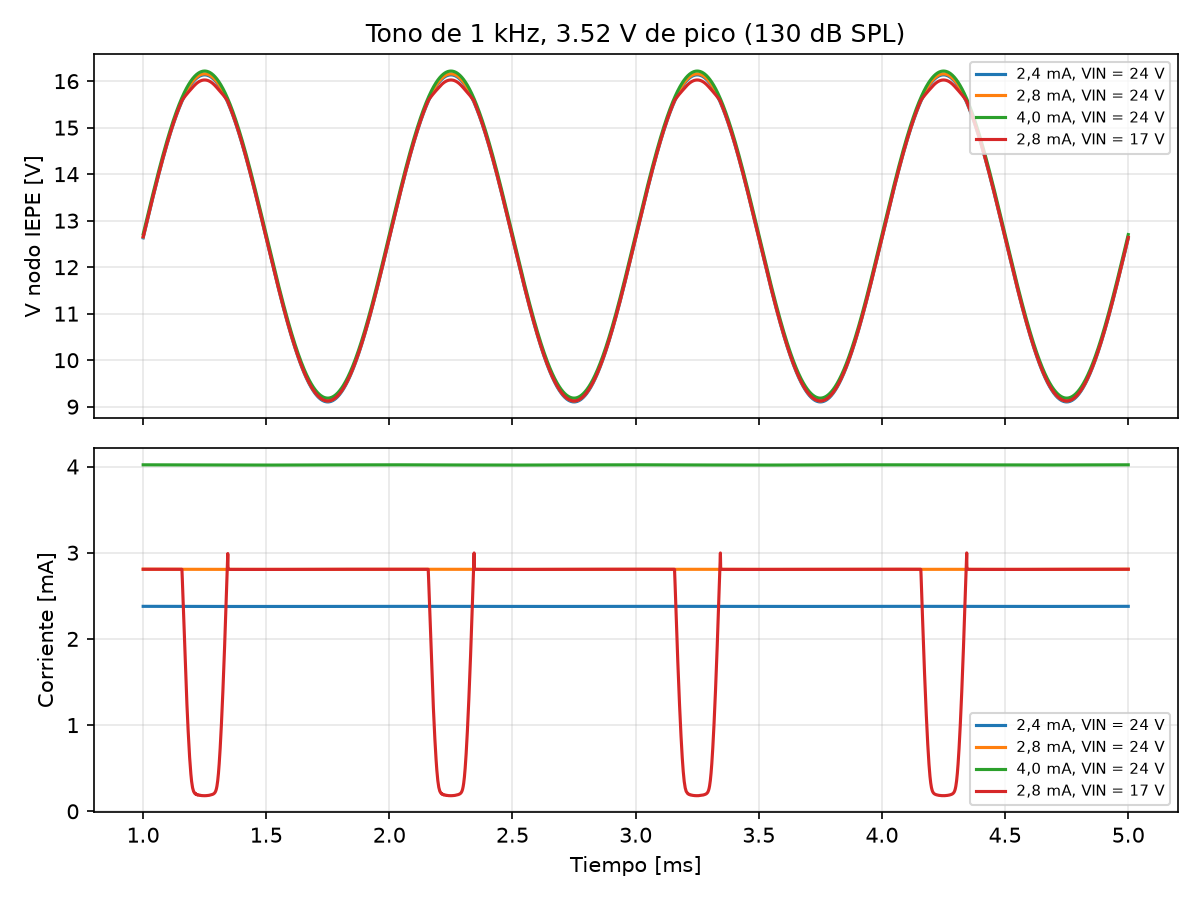
\includegraphics[width=\linewidth]{02_senal.png}
\captionof{figure}{Tensión y corriente con un tono al nivel máximo.}
\label{fig:senal}
\end{minipage}
\end{figure}

\textbf{Rizado de la alimentación (Fig.~\ref{fig:rizado}).} 50~mV de rizado a 120~Hz llegan a la señal como \textbf{0,13~$\mu$V}, unas 300 veces menos que el ruido del micrófono. A alta frecuencia la atenuación es menor, por lo que conviene una fuente lineal o filtrada.

\textbf{Ruido (Fig.~\ref{fig:ruido}).} Sin filtrar, la fuente añade 4~$\mu$V (10~\% del ruido del micrófono). Con un condensador de 100~nF junto a $R_{SET}$, como en el diseño de Analog Devices, baja a \textbf{0,46~$\mu$V} (1~\%).

\begin{figure}[H]
\centering
\begin{minipage}[t]{0.49\textwidth}
\centering
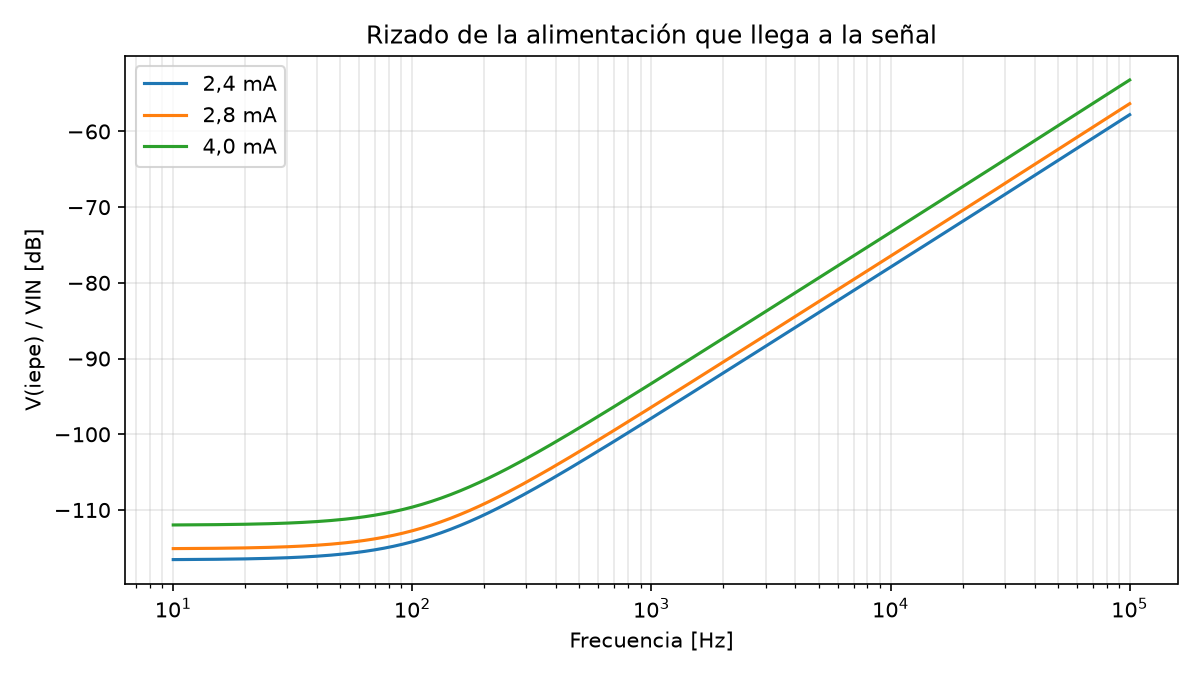
\includegraphics[width=\linewidth]{03_rizado.png}
\captionof{figure}{Fracción del rizado que llega a la señal.}
\label{fig:rizado}
\end{minipage}\hfill
\begin{minipage}[t]{0.49\textwidth}
\centering
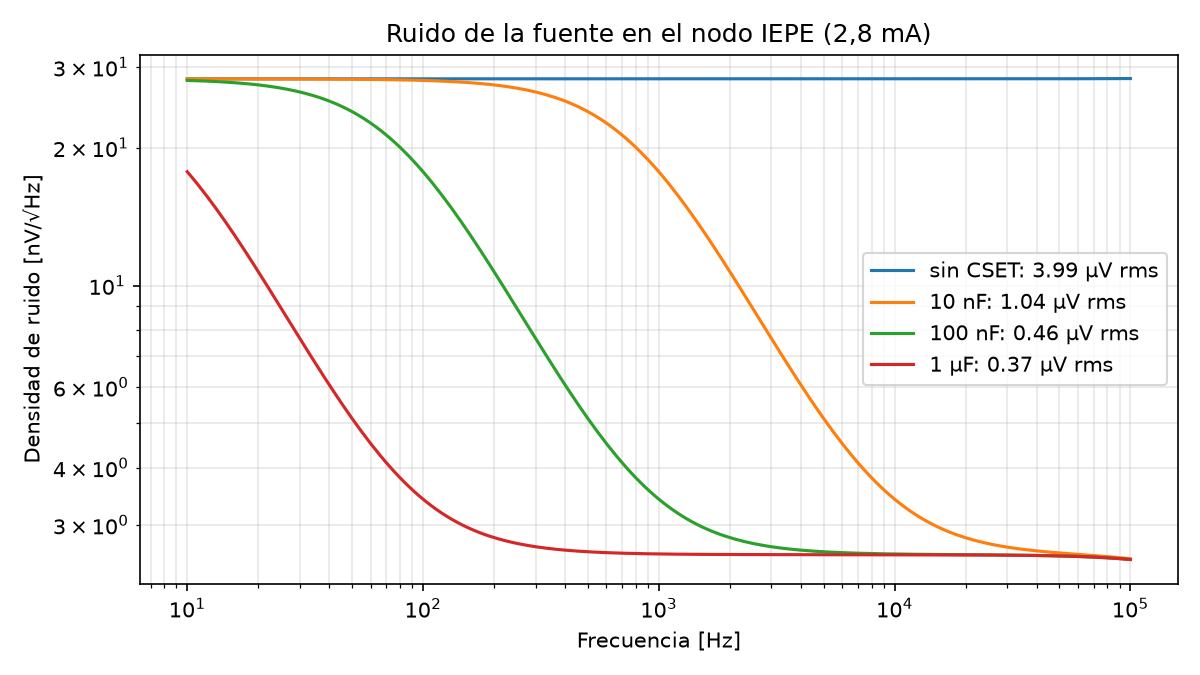
\includegraphics[width=\linewidth]{04_ruido.png}
\captionof{figure}{Ruido añadido según el condensador de filtrado.}
\label{fig:ruido}
\end{minipage}
\end{figure}

\begin{figure}[H]
\centering
\begin{minipage}[c]{0.49\textwidth}
\centering
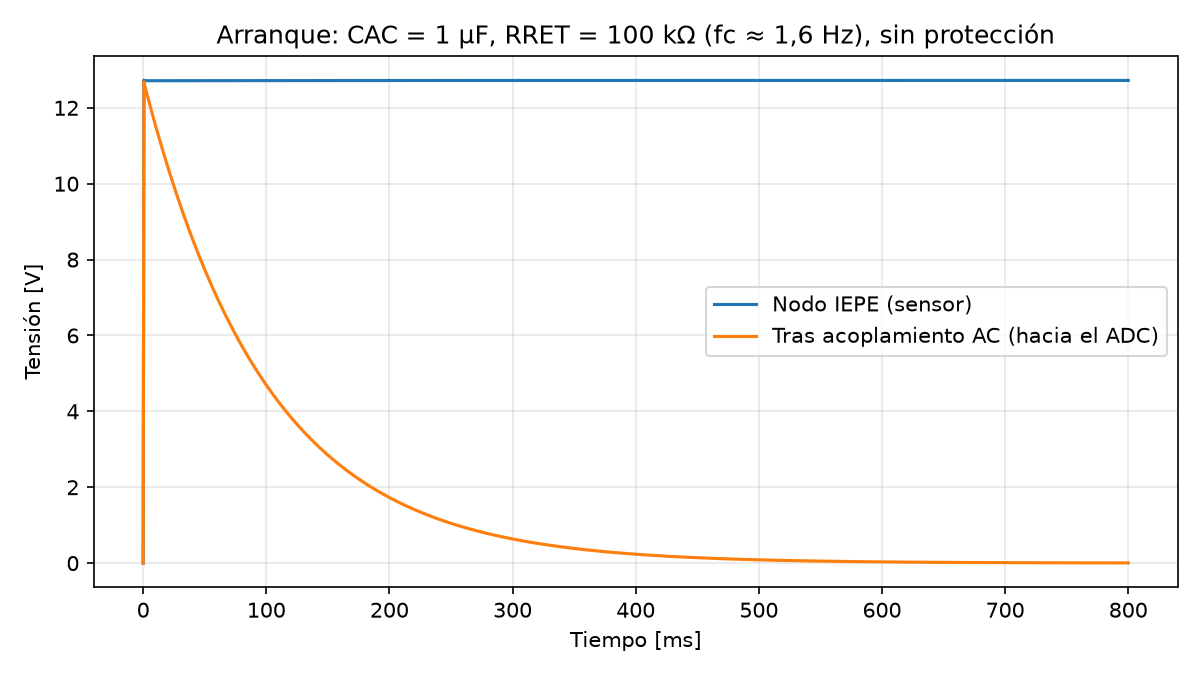
\includegraphics[width=\linewidth]{05_arranque.png}
\captionof{figure}{Tensión en el micrófono y tras el acoplamiento AC al encender.}
\label{fig:arranque}
\end{minipage}\hfill
\begin{minipage}[c]{0.47\textwidth}
\textbf{Encendido (Fig.~\ref{fig:arranque}).} Al conectar la alimentación, el salto de 0 a 12,5~V pasa momentáneamente por el acoplamiento AC: aparece un pico de \textbf{12,7~V} que desaparece en medio segundo. No es un defecto de la fuente, sino un requisito para la etapa siguiente, que necesitará protección.
\end{minipage}
\end{figure}

\section{Por qué la fuente aplica al proyecto}

\begin{table}[H]
\centering
\small
\caption{Requisitos del sonómetro y resultados de la simulación.}
\label{tab:resumen}
\begin{tabular}{p{6.6cm}p{6.4cm}c}
\toprule
Requisito & Resultado & ¿Cumple? \\
\midrule
Corriente entre 2 y 20 mA para el RG-50 & 2,4; 2,8 y 4,0 mA con error menor al 1 \% & Sí \\
Alimentación de 18 a 30 V sin recortar la señal & 24 V, con 6,4 V de margen sobre el máximo & Sí \\
Corriente estable con señales fuertes & Variación del 0,08 \% a 130 dB & Sí \\
Ruido menor que el del micrófono & 0,46 $\mu$V frente a 41 $\mu$V & Sí \\
Insensible al rizado de la red & 0,13 $\mu$V por cada 50 mV de rizado & Sí \\
Encendido seguro para la etapa siguiente & Pico de 12,7 V durante 0,5 s & Requiere protección \\
\bottomrule
\end{tabular}
\end{table}

La fuente cumple todos los requisitos que dependen de ella; el pico de encendido corresponde a la etapa siguiente y ya queda identificado. Configuración propuesta: \textbf{24~V, $R_{SET} = 20$~k$\Omega$, $R_{OUT} = 71{,}5~\Omega$ (2,8~mA) y un condensador de 100~nF} de película o cerámico C0G, porque otros cerámicos convierten las vibraciones en señal.

{\small
\begin{thebibliography}{9}
\setlength{\itemsep}{0pt}
\bibitem{roga} ROGA Instruments, \emph{RG-50 IEPE Microphone (1/4 in), hoja de datos}. \url{https://www.roga-instruments.com/downloads/PDF/RG-50-EN.pdf}
\bibitem{lt3092} Analog Devices, \emph{LT3092: 200 mA 2-Terminal Programmable Current Source}. \url{https://www.analog.com/en/products/lt3092.html}
\bibitem{cn0540} Analog Devices, \emph{CN0540: IEPE data acquisition signal chain}. \url{https://www.analog.com/en/resources/reference-designs/circuits-from-the-lab/cn0540.html}
\bibitem{tida010249} Texas Instruments, \emph{TIDA-010249}, TIDUF13, 2022. \url{https://www.ti.com/tool/TIDA-010249}
\bibitem{tida01471} Texas Instruments, \emph{TIDA-01471}, TIDUD62. \url{https://www.ti.com/tool/TIDA-01471}
\bibitem{ltspice} Analog Devices, \emph{LTspice}, versión 26.1.1. \url{https://www.analog.com/en/resources/design-tools-and-calculators/ltspice-simulator.html}
\end{thebibliography}
}

\end{document}
